\listfiles
\documentclass[preprint,5p]{elsarticle}
\usepackage[colorlinks=true,linkcolor=blue]{hyperref}%
\usepackage{todonotes}
\usepackage{booktabs}
\usepackage{amssymb}
\usepackage{acronym}
\usepackage{glossaries}
%\usepackage{lineno,hyperref}
%\modulolinenumbers[5]

\journal{None}



%%%%%%%%%%%%%%%%%%%%%%%
%% Elsevier bibliography styles
%%%%%%%%%%%%%%%%%%%%%%%
%% To change the style, put a % in front of the second line of the current style and
%% remove the % from the second line of the style you would like to use.
%%%%%%%%%%%%%%%%%%%%%%%

%% Numbered
%\bibliographystyle{model1-num-names}

%% Numbered without titles
%\bibliographystyle{model1a-num-names}

%% Harvard
%\bibliographystyle{model2-names.bst}\biboptions{authoryear}

%% Vancouver numbered
%\usepackage{numcompress}\bibliographystyle{model3-num-names}

%% Vancouver name/year
%\usepackage{numcompress}\bibliographystyle{model4-names}\biboptions{authoryear}

%% APA style
\bibliographystyle{model5-names}\biboptions{authoryear}

%% AMA style
%\usepackage{numcompress}\bibliographystyle{model6-num-names}

%% `Elsevier LaTeX' style
%\bibliographystyle{elsarticle-num}
%%%%%%%%%%%%%%%%%%%%%%%

\begin{document}

%%%%%%%%%%%%%%%%%%%%%%%%%%%%%%%%%%%%%%
%number of pca components
\newcommand{\pca}{25}
%length of templates before pcs
\newcommand{\prepca}{92}
%number of neurons in models
\newcommand{\nneurons}{200}
%number of connections
\newcommand{\nweights}{37 thousand}

\newcommand{\noise}{\mathcal{N}}
\newcommand{\noisefloor}{\mathcal{N}_f}
\newcommand{\stochasticnoise}{\mathcal{N}_s}
\newcommand{\db}{dB}


\newacronym{PCA}{PCA}{Principal Component Analysis}
\newcommand{\PCA}{\gls{PCA}} 

\newacronym{pc}{PC}{principal component}
\newcommand{\pc}{\gls{pc}} 
\newcommand{\pcs}{\glspl{pc}} 


%%%%%%%%%%%%%%%%%%%%%%%%%%%%%%%%%%%%%%

\begin{frontmatter}

\title{The low dimensional world of echolocating bats}

%\tnotetext[mytitlenote]{Fully documented templates are available in the elsarticle package on \href{http://www.ctan.org/tex-archive/macros/latex/contrib/elsarticle}{CTAN}.}

%% Group authors per affiliation:
%\author{Elsevier\fnref{myfootnote}}
%\address{Radarweg 29, Amsterdam}
%\fntext[myfootnote]{Since 1880.}

%% or include affiliations in footnotes:
%\author[mymainaddress,mysecondaryaddress]{Elsevier Inc}
%\ead[url]{www.elsevier.com}

%\author[mysecondaryaddress]{Global Customer Service\corref{mycorrespondingauthor}}
%\cortext[mycorrespondingauthor]{Corresponding author}
%\ead{support@elsevier.com}

%\address[mymainaddress]{1600 John F Kennedy Boulevard, Philadelphia}
%\address[mysecondaryaddress]{360 Park Avenue South, New York}

\begin{abstract}
This template helps you to create a properly formatted \LaTeX\ manuscript.
\end{abstract}

%\begin{keyword}
%\texttt{elsarticle.cls}\sep \LaTeX\sep Elsevier \sep template
%\MSC[2010] 00-01\sep  99-00
%\end{keyword}

\end{frontmatter}

%\linenumbers

\section{introduction}

Echolocating bats are long-lived, mobile animals. They use the landscape intensively for foraging, roosting, and commuting. They have excellent spatial memory \citep{Barchi2013,VonHelversen2005} and can rely on sonar to navigate to notable locations like foraging grounds, drinking places \citep[see][for references]{Vanderelst2016,Vanderelst2017}. Furthermore, bats have been reported to use sonar-based recognition of landmarks, both under experimental \citep{Jensen2005,Yu2019}, and natural \citep{Verboom1999} conditions.

Research on animal navigation has revealed a range of potential strategies that can be used to reach a distant goal \citep[Reviewed by][]{Franz2000}. Irrespective of the strategy an animal uses, a mechanism for recognizing previously visited places is required \citep{Vanderelst2016,Vanderelst2017}. This implies that echolocating bats can identify previously visited sites (or landmarks defining those places) using sonar. Currently, it is still an open question of how bats use sonar to recognize locations in the environment.

One mechanism for place recognition would be for bats to parse the stream of echoes returning from the environment into localized and identified objects \citep{Lee2017,Barchi2013,Moss2001,Schnitzler2003,Simmons2012,Ulanovsky2008,Clare2015,Surlykke2016}. However, as we argued before, it is highly questionable whether bats can interpret echoes in terms of a 3D environment model or acoustic image \citep[e.g.,][]{Vanderelst2015,Vanderelst2016,Steckel2013}. Sonar maps the three-dimensional structure of the environment on two one-dimensional waveforms arriving at the ears. While the time of arrival of echoes encodes object distance, azimuth and elevation directions are not directly available from the acoustic signal. In principle, azimuth and elevation can be estimated using spectral cues imposed by the head-related transfer function [REF]. However, complex environments, and even single plants [REF], return many overlapping and interfering echoes, making reconstructing the direction of origin of echoes much harder, and perhaps impossible. Extracting spatial information is further hampered by the limited temporal resolution of the sonar system \citep{Simmons1989,Wiegrebe1996,Surlykke1996}. 

We have suggested before that limitations of the bat's sonar system result in bats having access to a sparse, low dimensional description of the outside 3D world only \citep{Vanderelst2015a,Vanderelst2016}. Some recent evidence seems to confirm this. First, \citet{Geberl2019} confirmed that bio-sonar has a low spatial resolution, both for distance and angular dimensions. Also, neurophysiological data suggest that closely spaced objects are not perceived seperatly by echolocating bats. In contrast, neural responses to echo cascades from densely spaced objects seem to represent a single extended stimulus \citep{Warnecke2018}. \todo[inline]{Look at recent Simmons paper where bats refuse to fly through hoop}

Low dimensional descriptions potentially contain a lot of information \citep{Kuc1997b,Kuc1997}. We previously demonstrated that bats might use sonar template-based scene recognition \citep{Vanderelst2016,Vanderelst2017}. In this approach, bats are assumed to compare the acoustic signature of the environment to a set of previously stored signatures. We operationalized these acoustic signatures as time-intensity profiles, which could be derived directly from the cochlear output.

In this paper, we directly evaluate the hypothesis that sonar provides bats inherently with a low dimensional, yet sufficiently detailed, description of the world. We test this hypothesis in two steps. In a first step, we generate an extensive collection of synthetic echo sequences. We assess the compressibility of these echo signals using \PCA. Next, we filter the echo sequences using a model of the bat's auditory periphery \citep{Wiegrebe2008}. The synthetic echo sequences differ greatly in complexity. Nevertheless, the output of the cochlear model can be mapped onto a low-dimensional space. In a second step, we show that echoes collected in real bat habitats can be mapped into the same low-dimensional space, without loss of information. We do this by demonstrating that the low dimensional feature space allows recognizing locations in real habitats. 

Together these results suggest that echolocating bats live in a low dimensional perceptual world. The physics of the sonar system and the auditory periphery map the complexity of the 3D environment onto a small number of independent features, irrespective of whether we use artificial or real echo sequences. Nevertheless, this limited set of features is sufficiently rich for bats to recognize locations, and as we discuss, support flight control.

\section{Methods}

\subsection{Synthetic echoes}

In this section of the paper, we asses how the filtering in the auditory periphery reduces the complexity of input signals. We do this by presenting a simple generative model for echo sequences received by bats. Next, we assess whether the cochlear representation derived from these synthetic echo sequences can be projected into a low dimensional space. 

We created artificial echo sequences by randomly spacing ideal point reflectors. The distances of the point reflectors were selected using a two-step process. First we selected $n_{s}$ seed points $s$, uniformly distributed over a range from 0.5 to 7 meters. Next, for every seed point $s$, we selected $n_{c}$ cloud points normally distributed around $s$, with standard deviation 0.25 m. This two step process to modeling natural reflectors was inspired by the results of \citet{Yovel2009}, who found that echoes returning from vegetation could be better modeled using a similar two-step process than simply using uniformly spaced points. We generated xx sets of points for each combination of $n_s \in [xx,xx,xx, xx]$ and $n_c \in [xx, xx, xx, xx]$. Synthetic echoes consisting of few reflectors are likely to consist of only weak echoes. To ensure that all sequences included at least one strong echo, we added a single reflector at a distance between xx and xx to each collection of points.

Each set of points was converted to an impulse response with a sampling frequency $f_s$ of 219 kHz. The impulse response length was set to 7499 samples. These parameters correspond to the recording length and the sampling frequency used in the acoustic data collection (see below). In converting the point to an impulse response, we modeled attenuation of the echoes due to spherical spreading (both ways). We varied the amplitude of the impulses according to a normal distribution with a standard deviation of 10 dB. 

The impulse responses were converted to echo sequences by convolving them with a 1 millisecond long linear frequency-swept cosine starting at 100 kHz and ending at 40 Khz. Again, these parameters correspond to those used in the acoustic data collection described below. Examples of the resulting echo sequences are shown in figures \ref{fig:processing} and \ref{fig:synthetictemplates}. 

Artificial echo sequences were filtered using a model of the bat's auditory periphery, as proposed by \citet{Wiegrebe2008}. This model simulates the temporal and spectral resolution of the bat's cochlea. The model consists of a gammatone filterbank followed by half-wave rectification and non-linear compression. Finally, the model assumes a 1 kHz low-pass filter modeling the response characteristics of the inner hair cells. In the current implementation, we used a gammatone filterbank with xx filters, centered around xx kHz. The filters were spaced to correspond equivalent rectangular bandwidths \citep{Glasberg1990}.  The ouput of the channels were filtered with a time (distance) weighted factor corresponding to the atmospheric attenuation at the channel's center frequency. This filtering approximated frequency-dependent atmospheric attenuation. The first 6 ms of data were removed. This was done to ensure the data corresponded with the acoustic data. As indicated below, we removed the first 6 ms of those data to avoid including the pickup of the emitted signal. 

Figure \ref{fig:processing} depicts a single example of a synthetic echo sequence. It also illustrates the resulting response for each of the xx channels of the \citet{Wiegrebe2008} model. From these responses, it can be inferred that these are highly correlated. This is confirmed when analyzing the average cross-channel correlation for all xx synthetic echo sequences (Fig. \ref{fig:processing}xx). From these high cross-channel correlations, we conclude that the output of the cochlear model can be summarized by averaging across channels without extensive loss of information. An example of such a cross-channel sum is plotted in figure \ref{fig:processing}xx. In correspondence to our previous work \citep{Vanderelst2016}, we refer to this average across frequency channels as a template.

\begin{figure*}[tb]
	\centering
	\includegraphics[width=1\linewidth]{../results/processing}
	\caption{Example of synthetic echo sequence and its processing using the \citet{Wiegrebe2008} model. (xx) Example of a single synthetic echo sequence. (xx-xx) Response of the xx frequency channels in the \citet{Wiegrebe2008} model. From these plots, it can be seen that channels highly correlate. This is confirmed in panel xx, depicting the average correlation across channels for all xx synthetic echo sequences analyzed. (xx) The output of the \citet{Wiegrebe2008} model summed across the frequency channels, is referred to as a template in this paper. The template resulting from the echo sequence in panel xx is shown in panel xx. Panel xx shows the cumulative proportion of explained variance as a function of number of \pc\ across all templates for all synthetic echo sequences.}
	\label{fig:processing}
\end{figure*}

We used \PCA\ to assess the dimensionality of the templates generated from the synthetic echo sequences. We found that almost all of the variance in the templates could be captured by \pca\ components (see figure \ref{fig:processing}xx). Some examples of templates reconstructed from the principal components are shown in \ref{fig:synthetictemplates}xx).

\begin{figure*}[tb]
	\centering
	\includegraphics[width=1\linewidth]{../results/synthetic_templates}
	\caption{Example of synthetic echo sequences, their corresponding templates and the templates reconstructed from the \pca\ \pcs. (xx-xx) Three examples of synthetic echo sequence waveforms. Panels xx-xx depict the resulting templates (i.e., summation across the output channels of the \citet{Wiegrebe2008} model). These panels also show the result of projecting the templates into a \pca D space and transforming the result back to the original coordinates.}
	\label{fig:synthetictemplates}
\end{figure*}

In this section, we  used a generative model for naturalistic echoes. We assumed that echoes sequences received by bats can be considered as generated by anisotropically distributed point reflectors. Using this model, we have derived a low dimensional space ($D = \pca$), which can be used to describe the templates resulting from the artificial echo sequences. This implies that, after filtering through (a model of) the bat's auditory system, these artificial echoes can be converted to low dimensional descriptions. The original echo sequences, generated by xx to xx point reflectors effectively map to \pca\ dimensional vector. In the remainder of the paper, we will assess whether this low dimensional space allows describing the echoes from real bat habitats as collected using an ensonification device.

\subsection{Natural Templates}

\subsubsection{Acoustic data}

We reused the large library of echoes gathered in real bat habitats by \citet{Vanderelst2016}. Below, we briefly discuss the construction of templates based on these echoes, and we refer to our previous work for more details. \citet{Vanderelst2016} constructed an ensonification device featuring 31 Knowles FG series microphones connected to a custom-built sonar data acquisition board \citep{Steckel2013a}. The emitter was a Sensecomp 7000 Series ultrasonic broadband speaker. The ensonification device was mounted on a pan-tilt system allowing to rotate it in azimuth and elevation. The device and pan-tilt system was mounted on a tripod.

\begin{figure}[tb]
	\centering
	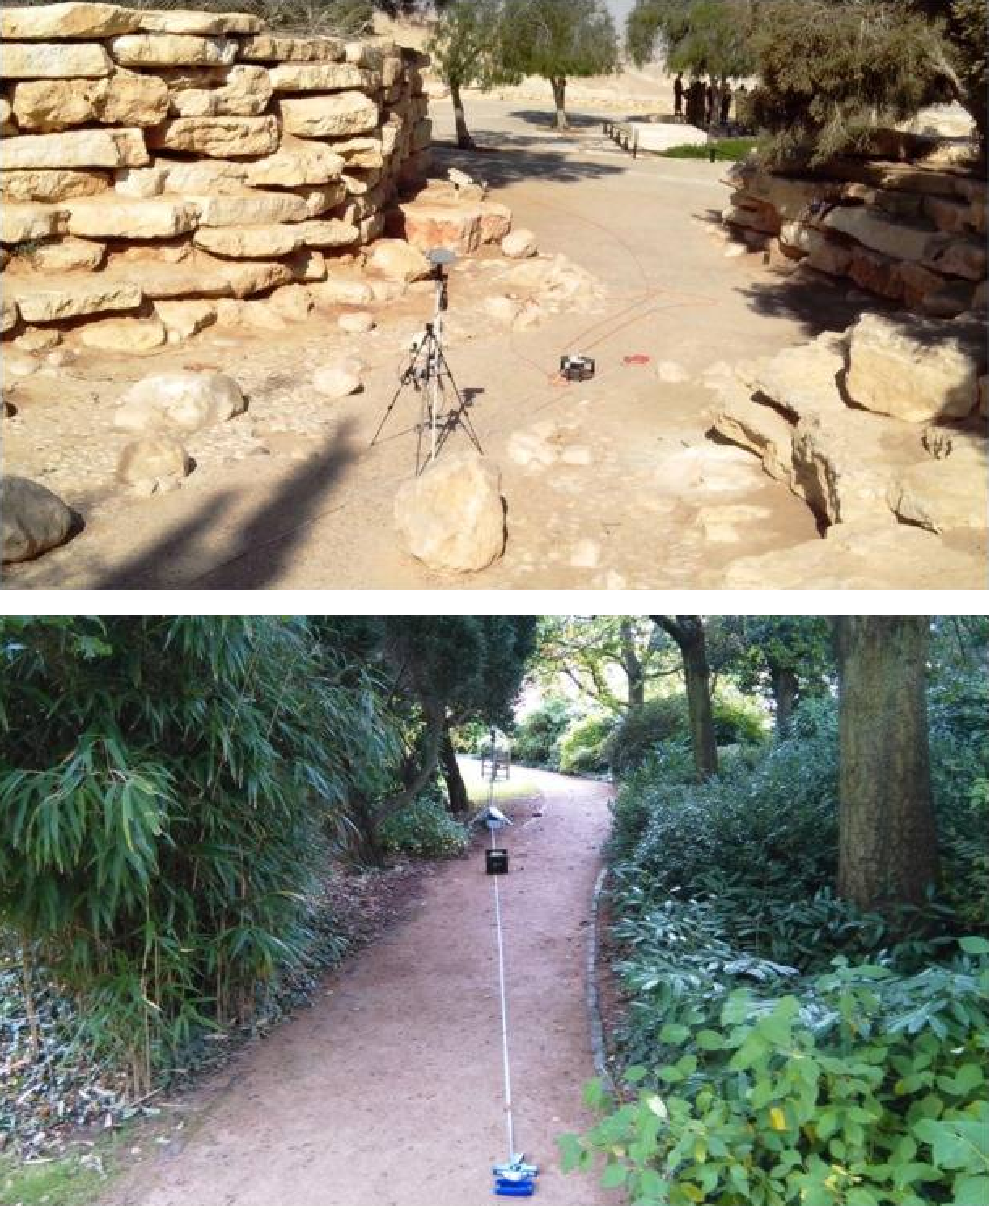
\includegraphics[width=1\linewidth]{figures/datacollection}
	\caption{Pictures of the sonar data acquisition process. Top: the ensonification device used at the Israeli site at Sde Boker. Bottom: The device used at the Bristol University Royal Fort Gardens. The tape measure indicated the transect along which the device was positioned in 40 steps.}
	\label{fig:datacollection}
\end{figure}

In our previous work, the ensonification device was used to ensonify bat habitats at three different sites. However, here we only use data collected along two linear pathways through natural habitats. At the first site, a public park in Sde Boker, Israel (Fig. \ref{fig:datacollection}). The environment consisted of a walkway lined with rocks and vegetation. Unpublished bat monitoring data at the site confirmed that bat used this corridor to commute. The ensonification device was placed at 50 positions along a straight line spanning a total of 10 meters Locations were spaced 20 cm apart. At each location, echoes were collected for 31 azimuth directions (-150 to +150 degrees) and 7 elevation directions (-40 to +25 degrees). Therefore, at each location, echoes were collected from 31 x 7 = 217 directions. At each azimuth and elevation direction, three repeat measurements were recorded. In this way, a total of 32,550 echo trains (50 positions x 217 directions x 3 repeats) for each of the 31 microphones in the device were collected.

The second site, at the University of Bristol Royal Fort Gardens (UK), data were collected at 40 different positions along a line (Fig. \ref{fig:datacollection}). Locations were spaced 25 cm apart. As for the Israel site, we collected data for 217 directions, and measurements were repeated three times. This resulted in 26,040 echo trains (40 locations x 217 directions x 3 repeats) for each of 31 microphones. The recording of the echoes started with the emission of a hyperbolic frequency modulated sweep and was recorded for 34 ms ($\sim$5.7 m) at a sampling rate of 219 kHz. 

\subsubsection{Template construction}

For every azimuth and elevation direction at each of the  40 or 50 locations, a biologically plausible acoustic signature of the environment was derived from the echoes, i.e., a template. Below, we briefly outline the steps used to derive templates from the acoustic data.

As we did for the synthetic echoes sequences, the echoes trains collected in bat habitats were filtered using a model of the bat's auditory periphery as proposed by \citet{Wiegrebe2008}. We concluded from analyzing the synthetic echoes that the response in different frequency channels is highly correlated. Therefore, the output of the cochlear model was averaged across frequencies to obtain a time-intensity profile, or template. The beam of the emitter used was more narrow than the typically combined hearing and emission directionality of bats \citep{Vanderelst2010a,Reijniers2010,Jakobsen2012}. Therefore, templates were averaged across three neighboring directions. The first 6 ms of data were removed to avoid using emitted signals for analysis. The processing steps outlined above resulted in 3 $\times$ 217 templates, for each location at each site, corresponding to 217 directions and three repeats.

Among the sets of templates, some had very little energy in them, notably those collected for directions without reflectors. For example, aiming the ensonification device upwards often resulted in no echoes returning. These templates could not be classified \citep{Vanderelst2016}. Therefore, we removed them from the current analyses by omitting all templates with very low energy. The resulting number of templates included in the present analyses are given in table \ref{tab:sizes}.

\subsubsection{Noise floor}

Internal (and, potentially, external) noise results in template values greater than zero, even in the absences of reflectors returning echoes. To avoid training the neural network on this noise, we estimated the noise floor in our data by collecting templates while pointing the device to empty space. The maximum template value obtained from these template measurements was used as the noise floor $\noisefloor$. The value of the noise floor $\noisefloor$ used had a numerical value of 0.15. Any template values below this value were set to this value. As we argued before \citep{Vanderelst2016}, using the empirical measurement noise to estimate $\noisefloor$ is biologically warranted as bats have a better signal to noise ratio in their auditory systems compared to our measuring device. Indeed, their dynamic range is at least 30 \db\ larger than our measurement device.

\subsubsection{Mapping templates into the \pca-dimensional space}

The templates from both sites were mapped into the \pca-dimensional space derived from the synthetic echoes, described above. We assessed how well the templates collected in real habitats can be represented by the \pca\ components by mapping the templates into this space and transforming the results back to the original space. Next, we calculated the correlation (and explained variance) between the original templates and the reconstructed templates.

\subsection{Artificial Neural Networks}

We wished to assess whether the templates projected into the \pca-dimensional space still contained sufficient information to be recognized. Previously, we assessed whether templates can be used to recognize locations using, what \citet{Baddeley2012} called, a perfect memory approach. Templates were stored in a lookup table. The Euclidean distance between two echo templates was the metric used to assess how well bats should be able to distinguish between templates. This table lookup and distance calculation require a comprehensive search of memory. Hence, in our previous work, we established that templates could be classified, but this required a significant amount of memory and computational resources.

Here, we used a more biologically plausible memory system: an artificial neural network. These are a neurally inspired way of distributed information storage in artificial neural networks \citep{Mcleod1998}. However, we acknowledge that current training methods most likely have no biological counterpart.

Simple artificial feedforward neural networks were implemented using Tensorflow 2 for Python. The first layer of the neural network added Gaussian noise to each input sample ($\sigma(\stochasticnoise) = 0.01$). The following layers were completely connected and used the rectified linear activation function. The output layer used a softmax activation function (or the normalized exponential function), normalizing the output into a probability distribution consisting of probabilities proportional to the exponentials of the output layer's activation. The loss was calculated as the cross-entropy between the target output and the actual output of the neural network. Weights were updated after each epoch using the Adam algorithm \citep{Kingma2014} .

For each site, we trained three neural networks, each taking the \pca-sample templates as input. The first neural network was trained to output the azimuth direction associated with the template (31 targets). The second network was trained to return the elevation (7 different targets). The final network returned the location (50 or 40 different targets). The targets for the network were encoded using the one-hot encoding scheme. 

Training a different neural network for each of these features ensured that the training algorithm paid equal attention to each feature. When training a single network for all features, the optimizer could preferably reduce errors in the location predictions as this feature has the largest variance. The full architecture can be considered as a single network with different streams for each feature (fig. \ref{fig:networks}).

We should point out that we did not take any steps to avoid so-called overfitting by the neural networks. Overfitting occurs when a neural network \citep{Ghotra2017}, or other mathematical models \citep{Hawkins2004}, extract complicated relationships between inputs and outputs that do not hold beyond the training examples. Overfitting typically reduces the ability of the model to generalize its predictive power to new data. However, in this case, the model is not required to generalize. Instead, we are only interested in whether the neural networks can learn and classify the set of training examples.

\begin{figure}
	\centering
	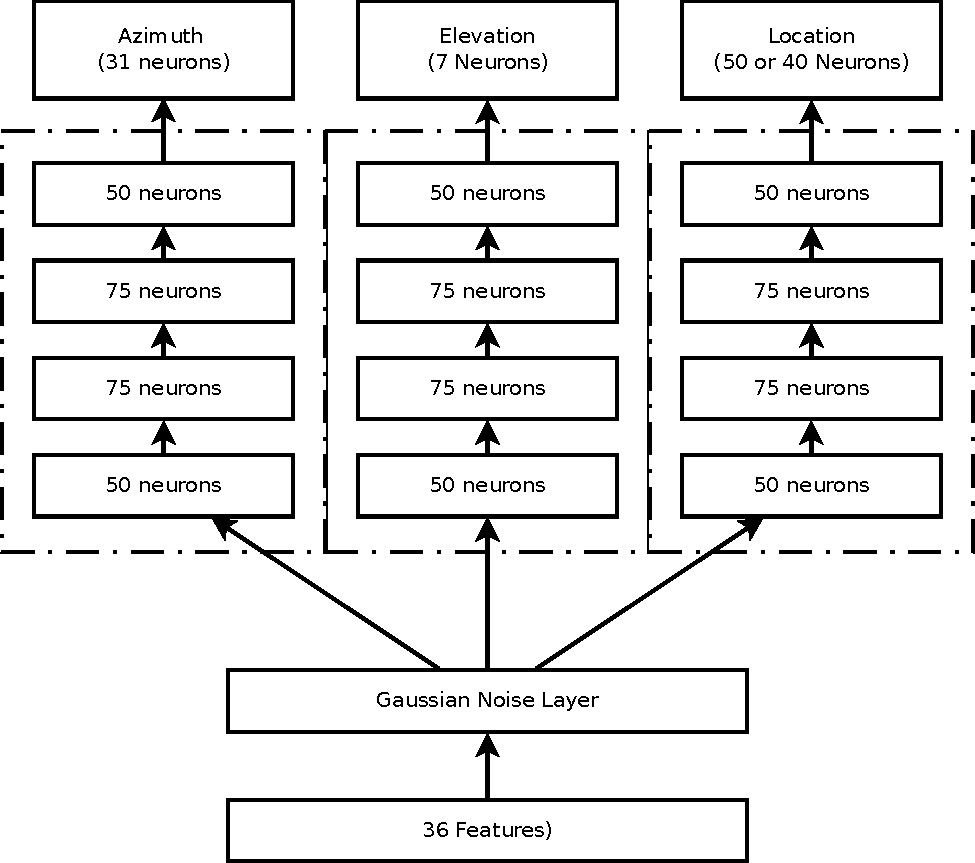
\includegraphics[width=1\linewidth]{figures/networks}
	\caption{Depiction of the neural network architecture trained for each site.}
	\label{fig:networks}
\end{figure}

\subsubsection{Training examples}

We wished to ensure that the neural networks encoded the templates and were able to recognize them in the presence of realistic noise. Indeed, it can be assumed that neural noise interferes with encoding or memorizing templates. Therefore, we trained the neural networks using templates to which noise was added.

In our previous work, we describe a procedure, based on \citet{Dau1996}, to derive a realistic model for stochastic noise. In brief, we empirically determined a noise level that resulted in a 75\% correct discrimination of two artificial bat calls differing by 2 \db\ in amplitude. This criterion is a conservative estimate of the just noticeable difference in loudness in bats. Based on this procedure we assumed internal (independent) Gaussian stochastic noise $\stochasticnoise$ for each sample with $\sigma(\stochasticnoise) = 0.01$ and $\mu=0$.

\subsection{Perfect Memory}

To be able to directly compare the results of the neural networks with the perfect memory approach \citep{Baddeley2012}, we implemented a version of the classification scheme employed in our earlier work \citep{Vanderelst2016}. We generated noisy templates by adding Gaussian noise to them ($\sigma(\stochasticnoise) = 0.01$). Next, we performed the classification of these noisy templates by finding the closest template (according to the Euclidean distance) in the original set of templates. The location, azimuth, and elevation of the closest template were considered as the noisy template's classification. This was repeated ten times, and we report on the average performance across these repeats.

\section{Results}

We found that the templates derived from acoustic data collected in real habitats could be well represented by the \pca\ components derived from synthetic data. This \pca-dimensional space could represent xx\% of the variance in the templates. Figure \ref{fig:empiricaltemplates} shows examples of templates and their reconstructed counterparts. Therefore, although the model used to generate echo sequences was very simple, the resulting underlying \pca D feature space could adequately represent templates resulting from real acoustic data.

\begin{figure*}[tb]
	\centering
	\includegraphics[width=1\linewidth]{../results/empirical_templates}
	\caption{Examples of three templates generated from the echoes collected at the Israel and Royal Fort Gardens site. The panels also depict the result of projecting the templates in the 
		\pca-dimensional space and transforming the result back to the original coordinates.}
	\label{fig:empiricaltemplates}
\end{figure*}

In our previous work \cite{Vanderelst2016}, we showed that the templates could be used to recognize locations in bat habitats. As we have shown that the templates can be projected into a lower \pca D feature space without loss, it can be expected that these \pca\ features can be used to locations as well. We found this to be indeed the case.

Figure \ref{fig:history} depicts the training history of all networks. This figure shows that, in all cases, training almost reached an asymptote around or before 250 epochs. However, some additional training can be seen up to xx epochs.



Figure \ref{fig:israelperformance} summarizes the performance of the three neural networks trained on the Israel templates. The performance was obtained by assuming that the most active output neuron represented the classification of the network. Inspecting the cumulative distribution of error reveals that the neural network encoding outperformed the perfect memory approach. The number of small errors was larger for the neural network than for the perfect memory. The neural network was able to classify about 70\% of templates with an error of fewer than 30 degrees in azimuth. In elevation, almost all templates were classified with an error below 15 degrees. Most (70\%) errors in location attribution were smaller than 0.5 meters. The confusion matrices confirm that most classification errors were small.

Interestingly, for azimuth and elevation, classification errors were not uniform across directions. This can be seen by the classification entropy plotted in figure \ref{fig:israelperformance}. In particular, these curves show interesting peaks around zero azimuth and medium elevations. The geometry of the environment can explain these peaks. The corridor (fig. \ref{fig:datacollection}) does not return a lot of echoes from azimuths around zero. Indeed, this direction is mostly open space. The same is true for elevations above 0. Elevations around 25 return very few echoes and this serves as a reliable indicator for classifying these templates, explaining the drop in entropy for elevation = 25 degrees.

\begin{figure*}
	\centering
	\includegraphics[width=1\linewidth]{../results/israel_results.pdf}
	\caption{Classification results for the Israel site. Top row: cumulative error distributions for the azimuth, elevation and location classification. Middle row: Confusion matrices for the classifications. Bottom row: remaining classification entropy for each target (derived from the confusion matrices).}
	\label{fig:israelperformance}
\end{figure*}

Figure \ref{fig:royalperformance} shows the results for the Royal Fort Park data. These results mirror those in figure \ref{fig:israelperformance}. Again the neural network outperformed the perfect memory approach by having more smaller errors. Overall, the performance for this data set was somewhat better than for the Israel data.

\begin{figure*}
	\centering
	\includegraphics[width=1\linewidth]{../results/royal_results.pdf}
	\caption{Simular as fig \ref{fig:israelperformance}, but for the Royal Fort Park site.}
	\label{fig:royalperformance}
\end{figure*}


\section{Discussion}

\subsection{The low dimensional world of bats}

\citet{Reijniers2010a} quantified the transmission of auditory information in the cochlea of bats. In that study, the authors adapted the Meddis inner hair cell model \citep{Meddis2006} to assess the amount of information in the acoustic signal preserved by the cochlea. These authors concluded that spectral notches introduced by overlapping echoes are faithfully encoded by auditory nerve
spike patterns. However, quantifying the information transfer rate also found that about half of the information (bits) are lost in the transduction from acoustic energy to spike trains. In the current paper, we expand on this work and quantify the dimension reduction due to cochlear encoding. Moreover, we show that this reduction in complexity still supports an ecologically valid task: sonar-based scene recognition.

We assumed echoes received by bats can be modeled as originating from a large collection of point reflectors. Passing these synthetic echoes through a model of the auditory periphery, we obtained a time-intensity profile (template) for each echo sequence. These templates could be well described by a low dimensional space of \pca\ principal components (figure \ref{fig:synthetictemplates}). We found that the same \pca D space could be used to describe templates originating from echoes collected in real bat habitats (figure \ref{fig:empiricaltemplates}). This suggests the filtering of the auditory periphery provides the bat with a greatly reduced acoustic description of its environment. To identify the locus of the compression, we performed a number of additional analyses. In particular, we evaluated whether the low-dimensional description is a property of the echo sequences, the gammatone filters, or the 1 kHz low-pass filter in the \citet{Wiegrebe2008} model.

We generated templates from the synthetic echo sequences using two versions of the \citet{Wiegrebe2008} model; with and without the 1 Khz low-pass filter. Per default, the model includes this filter to model the response characteristics of the inner hair cells \citep{Meddis2006,Reijniers2010a}. By removing this lowpass filter, we can assess to what extent it is responsible for the observed compressibility of the templates. We also generated templates using echo sequences of which the samples were randomly shuffled. This allows inferring whether the low-dimensionality of the templates is a property of the echo signals (before being filtered through the cochlear model). 

Figure \ref{fig:mechanism} shows the number of \pcs\ needed to capture 99\% of the templates variance. From this plot, it can be seen that the number of \pcs\ increases when shuffling the echo sequences increases from xx to xx. Omitting the 1 kHz filter from the  \citet{Wiegrebe2008} model increases the number of \pcs\ to xx.  Inspecting the average spectrum of the templates (fig. \ref{fig:mechanism}, inset) shows that most energy in the templates is contained in frequencies below 1 kHz. Therefore, it ought to be possible to completely represent templates by sampling them at 2 kHz,  or about 70 samples per template, as templates consist of 7499 samples at 219 kHz sample rate. This corresponds to the number of \pcs\ required to represent templates derived from echo sequences that were shuffled  (fig. \ref{fig:mechanism}). The number of \pcs\ required to represent unshuffled templates is about half of this, i.c., \pca. Therefore, we conclude that the 1 kHz filter is the main, but not exclusive, locus of the dimensionality reduction. The structure of the echo signals also increases the dimensionality of the templates.

\begin{figure}[tb]
	\centering
	\includegraphics[width=1\linewidth]{../results/mechanism}
	\caption{}
	\label{fig:mechanism}
\end{figure}

Despite the low dimensional character of the templates, they are sufficient to recognize environments. Indeed, this was demonstrated in our previous work \citep{Vanderelst2016}. Here, we directly demonstrated that the  \pca\ principal components are sufficient to discriminate their associated locations using neural networks.

Here, we show that a low dimensional signal is sufficient for recognizing environments. This is a critical component of navigation. However, bats do more than navigating. They also use sonar to control flight, for example, avoid obstacles or following guiding structures. The description the bat has access to for flight control has the same low-level character than that used for place recognition. Therefore, our work suggests that this low-level description is sufficient for flight control as well. We have shown before that a low-level description could be sufficient for obstacle avoidance and corridor following \citep{Vanderelst2015a,Mansour2019}. However, in that work, we converted both the echoes at the left and at the right ear to template-like representation. Subsequent work will have to demonstrate that the parameters of the \pca D space presented here can be used directly for controlling flight. In other words, we conjecture it should be possible to extract \pca\ features from an echo signal and convert this vector into a motor command. One can presume a neural network that converts the \pca\ features to flight control parameters.

\subsection{Template encoding}

We were unable to find numbers on the number of neurons in the cortex of bat species. However, the mouse cortex has been estimated to contain about $9 \cdot 10^4$ neurons or $7 \cdot 10^8$ synapses per cubic millimeter \citep{Braitenberg2013}. The neural networks presented in this paper consisted of about \nneurons\ neurons and \nweights\ connections. Therefore, in as much as these neural networks can be considered as biologically plausible models of memory, they are orders of magnitude smaller than a single cubic millimeter of mouse cortex. Let alone the complete cortex, which has been estimated to contain 75 million neurons \citep{Williams2000}. 

Despite their small size, the networks in this paper were able to encode (memorize) the templates as least as well as the perfect memory approach. The neural networks presented here are tiny compared to the density of cortical matter. However, the networks are also small compared to the data they encode. Table \ref{tab:sizes} lists the number of weights for the artificial neural networks and compares this number with the size of the \pca-dimensional templates. The number of floats making up the templates is larger than the number of weights by a factor of 2-3. Therefore, the networks have a smaller memory footprint than the data they encode. It should be noted that we have not made an attempt to try and to optimize (minimize) the size of the networks.

\begin{table}
	\centering
\begin{tabular}{lrrrrl}
	\toprule
	Site &       T &     n &      W &  W (nb\} &      R \\
	\midrule
	Israel &  206661 &  5299 &  53322 &   52425 &  25.8\% \\
	Royal &  302991 &  7769 &  51945 &   51075 &  17.1\% \\
	\bottomrule
\end{tabular}
	\label{tab:sizes}
	\caption{Table indicating the size of both template data sets and number of weights in the networks. The template size $T$ is obtained as $\pca \times n$, with $n$ the number of templates in the set. The number of weights $W$ includes all connections between neurons as well as the bias weights for each of the three networks trained. $W (nb)$ omits the bias weights. The ratio $R$ gives the ratio $W/T$.}
\end{table}


\subsection{Conclusion}

From our current work, in combination with previous results \citep{Vanderelst2016,Vanderelst2015a,Mansour2019}, we conclude that the auditory periphery of bats maps complex echoes to a limited number of features. These features can be efficiently stored to recognize scenes. Moreover, we conjecture that a (binaraural) version of the features should allow for sonar-based flight control. As such, a view of echolocating bats living in a low dimensional sensory space emerges.

\bibliography{references}

\onecolumn
\appendix
\section{Supplementary material}

\begin{figure}[h]
	\centering
	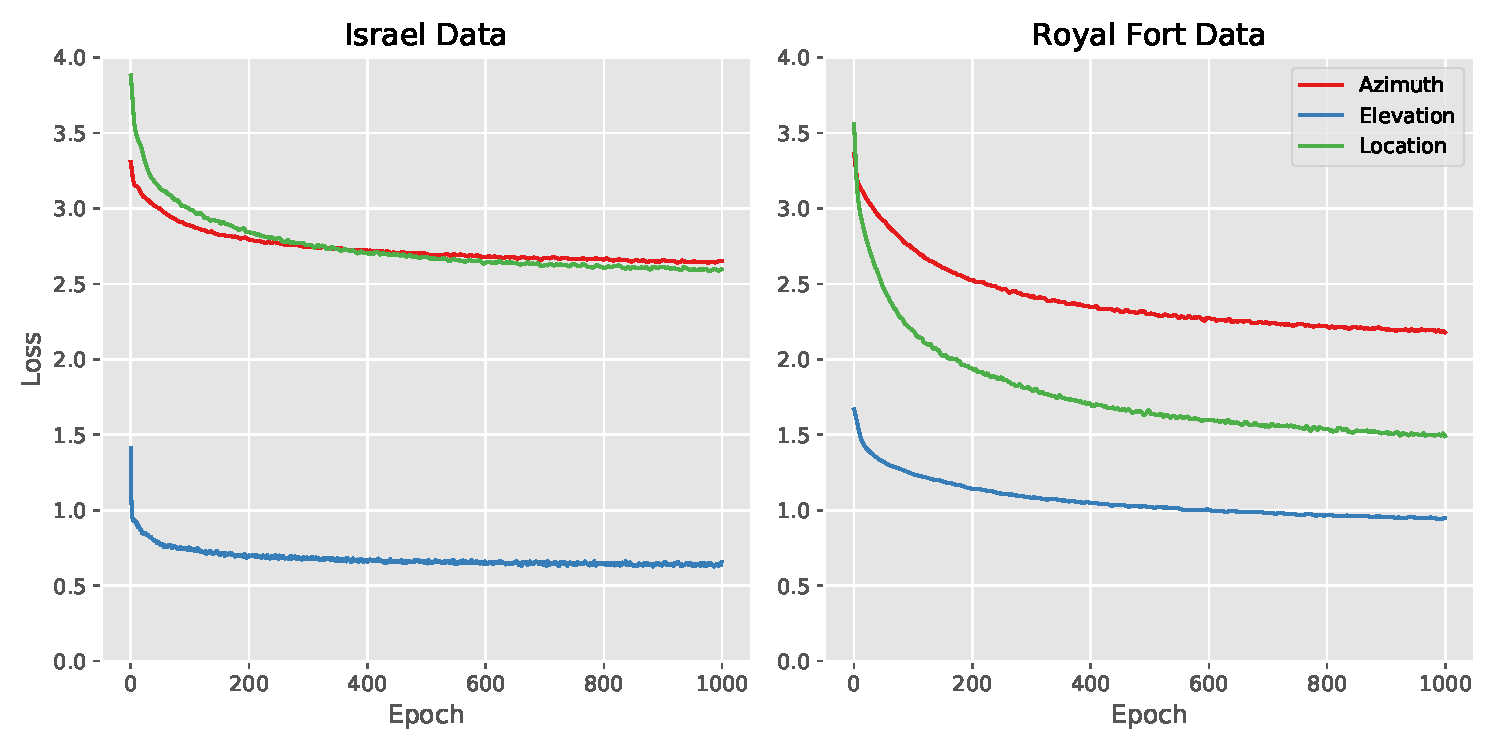
\includegraphics[width=1\linewidth]{../results/history}
	\caption{Training history of the neural networks. The plots give the value of the loss function as a function of training epoch. Notice the logarithmic x-axis.}
	\label{fig:history}
\end{figure}

\begin{figure}[h]
	\centering
	\includegraphics[width=1\linewidth]{../results/components}
	\caption{}
	\label{fig:components}
\end{figure}


\end{document}
